%
% File naacl2019.tex
%
%% Based on the style files for ACL 2018 and NAACL 2018, which were
%% Based on the style files for ACL-2015, with some improvements
%%  taken from the NAACL-2016 style
%% Based on the style files for ACL-2014, which were, in turn,
%% based on ACL-2013, ACL-2012, ACL-2011, ACL-2010, ACL-IJCNLP-2009,
%% EACL-2009, IJCNLP-2008...
%% Based on the style files for EACL 2006 by 
%%e.agirre@ehu.es or Sergi.Balari@uab.es
%% and that of ACL 08 by Joakim Nivre and Noah Smith

\documentclass[11pt,a4paper]{article}
\usepackage[hyperref]{naaclhlt2019}

\usepackage{times}
\usepackage{latexsym}

\usepackage{tabularx}
\usepackage{amssymb}
\usepackage{amsmath}
\usepackage{latexsym}
\usepackage{enumitem}
\usepackage{booktabs}
\usepackage{url}
\usepackage{color} 
\usepackage{verbatim}
\usepackage{calc}
\usepackage{arydshln}
\setlength\dashlinedash{0.7pt}
\setlength\dashlinegap{1.pt}
\setlength\arrayrulewidth{0.3pt}
\usepackage{mathtools}
\usepackage[draft,textsize=tiny]{todonotes}
\newcommand{\raq}[1]{\textcolor{blue}{R: #1}}
\newcommand{\marco}[1]{\textcolor{red}{M: #1}}
\newcommand{\gbt}[1]{\textcolor{green}{G: #1}}
\newcommand{\new}[1]{\textcolor{red}{#1}}
\newcommand{\redd}{Reddit$_{13}$}
\usepackage{soul}



%\aclfinalcopy % Uncomment this line for the final submission
%\def\aclpaperid{***} %  Enter the acl Paper ID here

%\setlength\titlebox{5cm}
% You can expand the titlebox if you need extra space
% to show all the authors. Please do not make the titlebox
% smaller than 5cm (the original size); we will check this
% in the camera-ready version and ask you to change it back.

\newcommand\BibTeX{B{\sc ib}\TeX}

%\title{Short-term meaning shift: an exploratory distributional
%analysis}
\title{Short-term meaning shift: a distributional exploration}

\author{First Author \\
  Affiliation / Address line 1 \\
  Affiliation / Address line 2 \\
  Affiliation / Address line 3 \\
  {\tt email@domain} \\\And
  Second Author \\
  Affiliation / Address line 1 \\
  Affiliation / Address line 2 \\
  Affiliation / Address line 3 \\
  {\tt email@domain} \\}

\date{}

\begin{document}
\maketitle
\begin{abstract}
We investigate diachronic meaning shift that takes place in short periods of time (short-term meaning shift) and in an online community of speakers. We create a small dataset and use it to assess the performance of a standard model for meaning shift detection on short-term meaning shift, and find that this phenomenon poses specific difficulties for models based on the Distributional Hypothesis. 
\end{abstract}

%============================
\section{Introduction}
\label{sect:Introduction}

Semantic change has received increasing attention in empirical Computational Linguistics / NLP in the last few years \cite{tang2018state}. Almost all studies so far have focused on meaning shift in long periods of time --decades to centuries. However, the genesis of meaning shift and the mechanisms that produce it operate at much shorter time spans, ranging
from the online agreement on words meaning in dyadic interactions \cite{brennan1996conceptual} to the rapid spread of new meanings in relatively small communities of people \cite{wenger2000communities,eckert-mcconnellginet1992}.\todo{M: substituted our cit. with more linguistic thing, so to be more consistent with what we say next}
\new{This paper is, to the best of our knowledge, the first exploration of the latter phenomenon---which we call \textit{short-term meaning shift}---using distributional representations.}
%\gbt{can we say it like this? else say ``with distributed representations'', or something} 
%\todo{R: empirical CL/NLP sounded weird to me here. Changed}
 
%in empirical CL/NLP, which we call \textit{short-term meaning shift}.

%\gbt{I change the order of the paragraphs}
%\todo{R: I would remove ``what seems to us''. Instead: As a first step in this direction, we analyze...}
%We \new{take what seems to us a natural first step, namely, to} analyze the
As a first step in this direction, we analyze the
 behavior of a standard distributional model of semantic change when
 applied to short-term shift.
This kind of model is based on the hypothesis that a change in context of use mirrors a change in meaning.
Our results show that a distributional successfully detects most short-term meaning shifts, but that it overgeneralizes, since some contextual changes do not correspond to a meaning shift.
%\gbt{this is the main result; I would not mention the false negatives cause they are very few.}
We also show that this is a difficulty caused by the nature of short-term meaning shift, and propose to use contextual variability as a means to remedy it.

\gbt{to do: We also should mention that we compare what we find to long-term shift.} \marco{I am not sure I understand what comparison you are referring to}

Short-term shift is usually hard to observe in standard language, such
as the language of books or news, which has been the focus of
long-term studies \cite{hamilton2016diachronic,kulkarni2015statistically}, since
it takes a long time for a new meaning to be widely accepted in the standard language. 
We therefore focus on the language produced in an online community of speakers, in which the 
adoption of new meanings happens at a much faster pace \cite{Clark96,hasan2009}.

% gbt: from the reviewer response (putting this here to give it prominence):
Unlike studies of long-term meaning shift, we cannot rely on material previously gathered by linguists or lexicographers for analysis or evaluation.
For this reason, we create a small dataset to enable empirical analysis of short-term
shift and to allow comparison in future studies.\footnote{Data and code will be made available upon
publication.}





% \marco{but
% also that, on the one hand, a change in context of use - as measured
% by cosine distance between the vector representations for a word at different periods of time
% does not always correspond to a meaning shift and, on the other hand, a meaning shift can take place also without a change in context of use. These results challenge the Distributional Hypothesis itself, which is at the basis of distributional / word embedding approaches to language in Computational Linguistics.}\todo{note: R thinks this paragraph should be the last cause it is rhetorically more powerful than the one below.}

% \marco{Finally, we investigate the role of \textit{contextual variability}, i.e. the extent to which a word tends to occur in a large set of contexts, and show that it provides valuable information which is complementary to the one about cosine distance for the detection of meaning shift on the short term.} 

%but also overgeneralises to words that exhibit an increase in frequency but no meaning shift. This challenges the Distributional Hypothesis itself, which is at the basis of distributional / word embedding approaches to language in Computational Linguistics.

%\marco{moved the paragraph to the conclusion.}
%While preliminary, our investigation opens the way to a new line of
%research within diachronic studies in our field, focusing on
%Short-term Meaning Shift originated and spread in small communities
%of speakers. Besides being of intrinsic theoretical interest, such a
%phenomenon has practical implications for every NLP downstream task
%concerning online communities, as modeling how words change their
%meaning in each community should allow a better understanding of the
%contents produced by its members.

%we study something new: meaning shift in a (relatively) short span. Main contributions:
%manually annotated dataset and analysis of the performance of current models.

%*** Our goal is to assess the performance of NLP system for long term shift detection on a short period. 

%Things to stress: in the nlp field, large work has been carried out on long term meaning shift (actually, when talking about meaning shift, the long term one - 'gay' example - is the only one considered). However, there exists also another kind on of shift, which is on the short term. While the long term meaning shift is observed at the level of general lanaguage, meaning that the new meaning o a word is gradually spread at all the levels of a (national?) community of spekaers, short term changes can not be observed at the same level, because, by their nature, they originate and are shared by smaller communities of speakers. Only if they manage, at some point, to go beyond that community and spread in other, they can be modelled as long term shifts (in the same way of 'gay'). So, in a way, exploring short term changes means looking at the genesis of the ones investigated in the nlp field up to know.

%We need to say which are the kind of shifts observed, and for this we need some theoretical framework. In any case, we have for sure memes,  referential phenomena and some kind of metaphorical process. 

%we need to say that we want also to observe how model for long term meaning shift work on this dataset. 

%%% Local Variables:
%%% mode: plain-tex
%%% TeX-master: "main"
%%% End:

 
%============================
\section{Related Work}
\label{sect:Related_Work}

Distributional models of semantic change are based on the hypothesis
that a change in context of use mirrors a change in meaning.
This in turn stems from the Distributional Hypothesis, that states
that similarity in meaning results in similarity in context of use \cite{harris1954distributional}.
Therefore, all models (including ours) spot semantic shift as a change in the word representation in different time periods.
This includes classic distributional representations obtained with count-based models, topic
modelling or Latent Semantic Analysis
\cite{sagi2011tracing,jatowt2014framework,wijaya2011understanding,gulordava2011distributional}
as well as more recent, neural-network based word embeddings
\cite{kim2014temporal,kulkarni2015statistically,hamilton2016diachronic,azarbonyad2017words,szymanski2017temporal,yao2018dynamic} %,del2016tracing}.
Note, however, that distributional representations from different time periods 
are not easily comparable.
We adapt the method by \newcite{kim2014temporal} to enable comparison
(see Section~\ref{sec:setup}).

Unlike previous work, we focus on the language of social communities.
Recent studies of this type of language have investigate the spread of new forms and meanings~\cite{del2017semantic,del2018road,stewart2018making}, 
competing lexical variants \cite{rotabi2017competition}, and the relation between conventions in a community and 
the social standing of its members \cite{danescu2013no}. 
None of these works has analyzed the ability of a distributional model to capture these phenomena, 
which is what we do in this paper for short-term meaning shift. 

Evaluation of semantic shift is difficult, due to the lack of
annotated datasets \cite{frermann2016bayesian}. For this reason, even for long-term shift, evaluation is usually performed by manually
inspecting the $n$ words whose representation changes the most
according to the model under investigation~\cite{hamilton2016diachronic,del2016tracing,kim2014temporal}.
Our dataset allows for a more systematic evaluation and analysis, and
enables comparison in future studies.

%% RAQ: Previous version
%\marco{While initial works focused on large periods (centuries), recently shorter time spans (decades) have been investigated \cite{szymanski2017temporal, yao2018dynamic}. However, the time span of these studies is still significantly larger than the one we consider here. Furthermore, these studies analyse data coming from newspapers, while we focus on language produced in an online community.}
%%\gbt{This is in contradiction with what we say in the intro -- we say there ``This paper is, to the best of our knowledge, the first exploration of the latter phenomenon—which we call short-term meaning shift—using distributional representations.'' Make consistent, please. Also, is the genre the only difference? (what about models or findings?)}
%Recent work has exploited language in social communities to investigate the adoption and spread of neologisms and new word meanings~\cite{del2017semantic,del2018road,stewart2018making}, the competition of different lexical variants \cite{rotabi2017competition}, and how the adoption of community conventions relates to the social standing of community members \cite{danescu2013no}. While providing insights on language variation, none of these works analyzed the ability of a distributional model to capture these phenomena, which is what we do in this paper for short-term meaning shift. 
%
%Evaluation of semantic shift is difficult, due to the lack of
%annotated datasets \cite{frermann2016bayesian}. For this reason, even for long-term shift, evaluation is usually performed by manually
%inspecting the $n$ words whose representation changes the most
%according to the model under investigation~\cite{hamilton2016diachronic,del2016tracing,kim2014temporal}.
%Our dataset allows for a more systematic evaluation and analysis, and
%enables comparison in future studies.




% gbt: shortened this cause we don't need as much detail
% Among the most widely used techniques are Latent Semantic Analysis
% \cite{sagi2011tracing,jatowt2014framework}, Topic Modeling
% \cite{wijaya2011understanding,rohrdantz2011towards}, and simple
% co-occurence matrices of target words and context terms 
% \cite{gulordava2011distributional,xu2015computational}.
% More recently, researchers have used word embeddings computed using the skip-gram model by \newcite{mikolov2013distributed}. Since embeddings computed in different semantic
% spaces are not directly comparable, time related representations are usually made comparable either by aligning different semantic spaces 
% %through a transformation matrix 
% \cite{kulkarni2015statistically,azarbonyad2017words, hamilton2016diachronic} or by initializing the embeddings at $t_{i+1}$ using those computed at $t_i$ \cite{kim2014temporal, del2016tracing,phillips2017intrinsic,szymanski2017temporal}. We adopt the latter methodology.


%RAQ: I have moved a revised version of this above, before the paragraph on evaluation
% b) previous work on meaning in communities
%\marco{Language variation in online communities has recently gained attention in NLP. Researchers have investigated the adoption and spread of neologisms and new words meanings~\cite{del2017semantic,del2018road,stewart2018making}, the competition of different lexical variants \cite{rotabi2017competition} and how the adoption of the linguistic conventions of a community is related to the social standing of the users within it \cite{danescu2013no}. While providing useful insights on language variation process, none of these works analyzed the performance of distributional models on it, which it is what we do in this paper.} 

%RAQ: this is going a bit too far for a short paper, so I commented it out
% a) previous work on short term meaning shift outside of CL
%\marco{Finally, we root our work in traditional studies from related fields such as sociolinguistics and psycholinguistics. In particular, our work is connected to the notion of of `communal common ground', defined as a set of meaning conventions developed in communities of sepakers \cite{Clark96}, and the one of `communities of practice' \cite{wenger1998communities,eckert-mcconnellginet1992}, used to indicate groups of individuals bound together by a common endeavour, and in which the sharing of common linguistic conventions is a key aspect for the construction of the group identity.}


%\todo{Important: pieces missing in the related work, in particular (a)
%  previous work on short term meaning shift outside of CL [mostly
%  theoretical linguistics I guess; difference to us:
%  method?], (b) previous work on meaning in communities (your work?)}
%
%\todo{I added a and b (in reverse order, b-a). However, I think a probably does not fit, and I would remove it.}


%####################################################
% OLD STUFF
%####################################################
%\raq{I find the last paragraph below a bit boring. The model is not our strong point, so no need to make this prominent. Instead I would highlight that previous work on LTMS is evaluated qualitatively or using judgements by the investigators. Instead, we use judgements by domain experts. }\todo{I agree with the change in emphasis, and also with Marco's remark that he'd like to keep this info. Marco, can you summarize and downplay the part about self-similarity and highlight what Raquel says?}
% ACL VERSION
%It is not straightforward to compute self-similarity across time with neural-based representations, since, due to the stochastic nature of the process, the embeddings computed in different semantic spaces are not directly comparable. Two main solutions have been proposed in the literature. The first consists in computing the embeddings separately for each time bin and then aligning different semantic spaces through a transformation matrix, that can be learned either employing linear regression \cite{kulkarni2015statistically,azarbonyad2017words} or orthogonal Procrustes \cite{hamilton2016diachronic}. The second type of solution,  introduced by \newcite{kim2014temporal}, is based on initializing new embeddings with existing embeddings. This methodology has been adopted in several recent diachronic studies\cite{del2016tracing,phillips2017intrinsic,szymanski2017temporal}, and we also adapt it for our purposes here.


%\gbt{Shouldn't you also cite your own previous work on meaning shift
%  in online communities?}

%Neural based work on diachronic meaning shift:\\
%\cite{kulkarni2015statistically,zhang2015omnia,hamilton2016diachronic}. stress
%that Hamilton says that emb are the best.\\ An alternative approach,
%which we also adopt - with a slight change - in our work, is
%introduced by \newcite{kim2014temporal}, who propose a simple but
%effective methodology to make vectors trained on different corpora
%directly comparable: embeddings created for year~$y$ are used to
%initialise the vectors for year $y+1$. The process is progressively
%applied to all time spans.\\ The SCAN model proposed by Frermann et
%al. (2016) is a dynamic Bayesian topic model.  EXPLANATOIN OF THE
%MODEL For each target word, a SCAN model is created that represents
%the meaning of the word with two distributions: a K-dimensional
%multinomial distribution over word senses φ and a V-dimensional
%distribution over the vocabulary ψ for each word sense. As a
%generative model, SCAN starts with a precision parameter κ , a Gamma
%distribution with parameters a and b that controls the extent of
%meaning change of φ. A three time step model involves the generation
%of three sense distributions φ , φ , and φ ,at times t-1, t and
%t+1. The sense distribution at each time generates a sense z, which
%in turn generates the context words for the target
%word. Simultaneously, for each time of t-1, t and t+1, the word-sense
%distributions ψ , , ψ , and ψ , are generated, each of which also
%generates the context words for the target word. The prior is an
%intrinsic Gaussian Markov Random Field which encourages smooth change
%of parameters at neighboring times. The inference is conducted with
%blocked Gibbs sampling.


%The phenomena of widening and narrowing are discussed in most
%studies, such as Sagi et al. (2009) and Gulordava et
%al. (2011). Novel senses, namely the birth of lexical senses are
%discussed in details in Erk (2006), Lau et al. (2012), Mitra et
%al. (2015), Frermann et al. (2016), Tang et al. (2016) and
%others. Pejoration and amelioration are dealt with in Jatowt et
%al. (2014)

%%% ******** FROM CLIC 16 PAPER ********
%The automatic modelling of diachronic shift of meaning has been investigated employing several different techniques. Among these, most recently, Latent Semantic Analysis \cite{sagi2011tracing,jatowt2014framework} and topic clustering \cite{wijaya2011understanding}.
%Vector representations for diachronic shift of meaning have been used by \newcite{gulordava2011distributional}, with a simple co-occurence matrix of target words and context terms. \newcite{xu2012computational} and \newcite{jatowt2014framework} experimented both with a bag-of-words approach and a more linguistically motivated representation that also captures %not only the frequency of co-occurring words but also 
%their relative positions in relation to the target word. 
%%who build 
%%context vectors for target words using simple co-occurrence matrix, where row elements are target words and column elements are context terms, and then apply local mutual information (LMI) to the matrix. Similar representations have been employed also by 
%
%Recently Word Embedding (see 4.4) have been used to investigate diachronic meaning shift: 
%%When using word embeddings \note{do we need to introduce the term?} to investigate diachronic meaning shift, 
%vectors are usually created independently for each time span and are mapped from one year to another via a transformation matrix, as %a transformation matrix is used to map vectors from one year to another %.  Indeed, even if there isn't an absolute correspondence between vectors in different semantic spaces, 
%the relative positions of vectors in different spaces are stable 
%\cite{kulkarni2015statistically,zhang2015omnia,hamilton2016diachronic}.
%%, \note{FIX: and thus a linear (Wt′  →t (w) ∈ Rd×d) that maps a word from φt to φt′ is feasible.}
%%These approaches are based on the idea that a transformation matrix can be learnt .... \note{mettere un po' di math: io direi solo spiegare in due parole} 
%%and also by \cite{}, who use the orthogonal Procrustes to align the learned embeddings of different periods.
%%%%%% THIS WAS A NICE BIT, BUT RELATED IS TOO LONG
%%A similar model is used by \newcite{zhang2015omnia}, who introduce the concept of ``global similarity'' as the correspondence across years between terms 
%%(``walkman'' and ``iPod'', e.g.)
% %that share similar contexts, found using a transformation matrix for vectors in different periods. 
%%In addition to this, they also compute a "local similarity", i.e. they also take into consideration the cosine similarity with some reference points in the synchronic semantic space.
%An alternative approach, which we also adopt - with a slight change - in our work, is introduced by \newcite{kim2014temporal}, who propose a simple but effective methodology to make vectors trained on different corpora directly comparable: embeddings created for year~$y$ are used to initialise the vectors for year $y+1$. The process is  progressively applied to all time spans.
%
%
%
%%\newcite{tahmasebi:15} identify three types of language change: the first one is spelling variation, the second one is what they name \textit{term to term evolution}, where different words are used to refer to the same concepts over time, including named entities. This class comprises cases such as ``The Great War'' and ``World War I'', or ``fine" which in the past was used in the same was as now is ``foolish". The third type they identify is \textit{word sense evolution}. 
%
%%In order to find word to word evolution, words are mapped to concepts (word senses), and then the context of concepts is compared. 
%
%
%%Instead, to find general word to word evolution, word senses must be used. A word is first mapped to a concept representing one of its word senses at one point in time. If one or several other words point to the same concept largely at the same period in time, then the words can be considered synonyms. If the time periods do not overlap, or only overlap in a shorter period, the words can be considered as temporal synonyms or word to word evolutions.
%
%%% see also: (context-based approach) Sagi, E., Kaufmann, S., Clark, B.: Semantic density analysis: comparing word meaning across time and phonetic space. In: Workshop on Geometrical Models of Natural Language Semantics, GEMS 2009, pp. 104–111 (2009). http://dl.acm.org/citation.cfm?id=1705415.1705429
%%% methods making use of probabilistic topic models:
%% Lau, J.H., Cook, P., McCarthy, D., Newman, D., Baldwin, T.: Word sense induction for novel sense detection. In: Conference of the European Chapter of the Association for Computational Linguistics, EACL 2012, pp. 591–601 (2012). http://aclweb.org/anthology-new/E/E12/E12-1060.pdf
%%% Wijaya, D.T., Yeniterzi, R.: Understanding semantic change of words over centuries. In: Workshop on DETecting and Exploiting Cultural diversiTy on the social web, DETECT 2011, pp. 35–40 (2011). doi:10.1145/2064448.2064475

%%% Local Variables:
%%% mode: latex
%%% TeX-master: "main"
%%% End:

%============================
\section{Experimental Setup}
\label{sec:setup}


% === DATA ==============

\paragraph{Data.}
We exploit user-generated language from an online forum of football fans,
namely, the r/LiverpoolFC subreddit, one of the many communities hosted
by the Reddit platform.\footnote{\url{https://www.reddit.com}.}
%\marco{I would remove this link, it is useless} 
%\raq{We can consider this at the end.}
We focus on a short period of eight years, between 2011 and 2017. 
In order to enable a clearer observation of short-term meaning shift, we define two
non-consecutive time bins: the first one ($t_1$) contains data from
2011--2013 and the second one ($t_2$) from 2017.\footnote{These choices
  ensure that the samples in these two time bins are approximately of the same size -- see Table~\ref{tab:data}. The
  r/LiverpoolFC subreddit exists since 2009, but very little content
  was produced in 2009--2010.}
 We also use a large sample of community-independent language for the
initialization of the word vectors, namely, a random crawl from Reddit
in 2013.\footnote{We used the Python package Praw for downloading the data, \url{https://pypi.python.org/pypi/praw}.} Table~\ref{tab:data} shows the size of each sample.

%----- TABLE ----------------------------------------------------
\begin{table}[t]\small
\centering
\begin{tabular}{lccc}
\bf sample & \bf time bin & \bf million tokens \\
 \hline
\redd &  2013 & {\raise.17ex\hbox{$\scriptstyle\sim$}}900 \\
LiverpoolFC$_{13}$ & 2011--13 & ~ 8.5\\
LiverpoolFC$_{17}$ & 2017 & 11.9\\ \hline
\end{tabular}
\caption{Time bin and size of the datasets.}
\label{tab:data}
\end{table}
%----- END TABLE -----------------------------------------



%=== MODEL ==========

\paragraph{Model.}
%We adapt the methodology introduced by 
%, which in turn builds on the skip-gram architecture by \newcite{mikolov2013distributed}
In the method proposed by \newcite{kim2014temporal}, word
embeddings for the first time bin $t_1$ are initialized randomly; then,
given a sequence of time-related samples, embeddings for $t_i$
are initialized using the embeddings of $t_{i-1}$ and further
updated. 
%with the standard skip-gram architecture.
If at $t_i$ the word is used in the same contexts as in $t_{i-1}$, its embedding will only be marginally updated, whereas a major change in the context of use will lead to a stronger update of the embedding. The model makes embeddings across time bins directly comparable.

%Recall that we want to spot changes that occur between 2013 and 2017 (the latter included). Since training directly on LiverpoolFC$_{13}$ is not possible due to data sparseness, 
We implement the following steps:
First, we create  randomly initialized word embeddings with the large sample \redd, to obtain meaning
representations that are community-independent.
%\footnote{\redd\ embeddings are initialized randomly.} \marco{Useless footnote, we say about the random initialization before}
We then use these embeddings
to initialize those in LiverpoolFC$_{13}$, update the vectors on this
sample, and thus obtain embeddings for time $t_1$. This step
adapts the general embeddings from \redd\  to the
LiverpoolFC community. Finally, we
initialize the word embeddings for LiverpoolFC$_{17}$ with those of $t_1$, train on this sample and get embeddings for $t_2$.\footnote{We implement the model
using the \texttt{gensim} library.}   
%To obtain word embeddings for time $t_2$, we
%initialize the word embeddings for LiverpoolFC$_{17}$ with those of $t_1$, 
%and train skip-gram further on the
%LiverpoolFC$_{17}$ data.

%We define the vocabulary to be represented as the intersection of the vocabularies of the three samples (\redd, LiverpoolFC$_{13}$, LiverpoolFC$_{17}$) which results in a vocabulary of 157k words.

The vocabulary is defined as the intersection of the
vocabularies of the three samples (\redd, LiverpoolFC$_{13}$,
LiverpoolFC$_{17}$), and includes 157k words.
%\todo{What is the vocabulary size?} 
%\redd~embeddings are initialized randomly. 
For \redd, we include only words that occur at least 20 times in the
sample, so as to ensure meaningful representations for each word,
while for the other two samples we do not use any frequency
threshold: Since the embeddings used for the initialization of
LiverpoolFC$_{13}$ encode community-independent meanings, if a word doesn't occur in
LiverpoolFC$_{13}$ its representation will simply be as in \redd,
which reflects the idea that if a word is not used in a community, then its meaning is not altered within
that community. 
%Instead, if a word's meaning changes in the
%community, then we expect the word embedding to change accordingly
%after training on the community-specific data.
%Analogous reasoning applies to LiverpoolFC$_{17}$. 
We train with standard skip-gram parameters \cite{levy2015improving}: window 5, learning rate 0.01, embedding dimension 200, hierarchical softmax.


%===== EVALUATION DATASET ===============


\paragraph{Evaluation dataset.}

We create a small dataset of words to be annotated by members of the r/LiverpoolFC
subreddit, that is, community members with domain knowledge (needed for this task) but no linguistic background.
We initially leverage information about increase in frequency, which has been shown to positively correlate with meaning change \cite{wijaya2011understanding,kulkarni2015statistically}, and sample content words with a significant increase in relative frequency (at least two standard deviations above the mean) between $t_1$ and $t_2$. Frequency increase is not a necessary condition for meaning shift to take place; however, it is a reasonable starting point, as a random selection of words would contain very few positive examples. Our dataset is thus biased towards precision. 
This procedure yields $\sim$200 words. We then manually identified cases of semantic shift among these words, i.e., changes in the ontological type of what a word denotes (see examples in Section~\ref{sec:types}) by analyzing their contexts of use in the r/LiverpoolFC data. This resulted in 34 words. We added two types of confounders: 33 words with a significant increase in frequency but not marked as meaning shift candidates and 33 words with constant frequency between $t_1$ and $t_2$, included as a sanity check.\footnote{All words have absolute frequency in range [50--500].} 

%We then created an online survey, which we posted in the r/LiverpoolFC to recruit participants. 
The participants were shown the 100 words (in randomized order) together with randomly chosen contexts of usage from each time period ($\mu$=4.7 contexts per word) and, for simplicity, were asked to make a binary decision
about whether there was a change in meaning. However, semantic shift is arguably a graded notion, so we aggregate the annotations into a graded \emph{semantic shift index}, ranging from 0 (no shift) to 1 (shift) depending on how many subjects spotted semantic change.\footnote{The shift index is exclusively based on the judgements by the redditors, and does not consider the preliminary candidates selection done by us.}  Overall, 26 members of r/LiverpoolFC participated in the survey, and each word received on average 8.8 judgements. The final dataset includes 97 words.\footnote{Three words were discarded: `discord'  and `owls' due to the homonymy with proper names not detected during survey's implementation; `tracking' because the chosen examples clearly mislead the judgements of the redditors.} 
Further details are in the supplementary material.


%*** SHORT VERSION***

%\paragraph{Evaluation dataset.}  
%The dataset includes 97 words, which were annotated by 26 members of the r/LiverpoolFC
%subreddit, that is, community members with domain knowledge (needed for this task) but no linguistic background.
%For each word, subjects
%read contexts of use from the two time bins and, for simplicity, were
%asked to make a binary decision
%about whether there was a change in meaning. However, semantic shift
%is arguably a graded notion, so we aggregate the annotations into a
%graded \emph{semantic shift index}, ranging from 0
%(no shift) to 1 (shift) depending on how many subjects spotted
%semantic change. This index is shown in the y-axis of
%Figure~\ref{fig:shift-cosine}. Further methodological details regarding data
%collection are described in the supplementary material. 



%*** LONG VERSION ***

%\paragraph{Evaluation dataset.}\todo{M: I commented out the short version of the paragraph and put back the long/original one, with small additions - in red} 
%For evaluation and analysis, we create a small dataset of words to be annotated as positive or negative meaning shift examples by community members without linguistic background.\footnote{Domain knowledge is needed for this task.}
%We initially leverage information about increase in frequency, which has been shown to positively correlate with meaning change \cite{wijaya2011understanding,kulkarni2015statistically}, and sample words with a significant increase in relative frequency between $t_1$ and $t_2$ (an increase is considered significant if it is at least two standard deviations above the mean).\footnote{We consider   content words only, which we identify by using the external list of common words available at \url{https://www.wordfrequency.info/free.asp}} Frequency increase is not a necessary condition for meaning shift to take place; however, given the positive correlation mentioned above, it is a reasonable starting point, as a random selection of words would contain very few positive examples. Our dataset is thus biased towards precision. 
%This procedure yields $\sim$200 words. The first author of the paper went through the list of words to identify cases of potential meaning shift, based on the analysis of the contexts of use in the r/LiverpoolFC data. By semantic shift, we mean change in the ontological type of what a word denotes (see examples in Section \ref{sect:results}). We considered only new senses - i.e., not existing senses which increase in frequency- , both for monosemous and polysemous words. This resulted in 34 words. We added two types of confounders: 33 words with a significant increase in frequency but not marked as meaning shift candidates and 33 words with constant frequency between $t_1$ and $t_2$, included as a sanity check.\footnote{All words have absolute frequency in range [50--500].} 
%
%We then created an online survey, which we posted in the r/LiverpoolFC to recruit participants. The participants were shown the 100 words together with randomly chosen contexts of usage from each time period (1 to 5 contexts depending on the word - \textcolor{red}{mean number of contexts per word=4.7})). For feasibility, they were asked to label words as `shift' or `no shift', although semantic shift is better viewed as graded (see below). The order of presentation was randomized for each participant.\footnote{Survey's instructions are in the supplementary material.} Overall, 26 members of r/LiverpoolFC participated in the survey, and each word in the dataset received on average 8.8 judgements. The final dataset includes 97 words.\footnote{Three words were discarded: `discord'  and `owls' due to the homonymy with proper names not detected during survey's implementation; `tracking' because the chosen examples clearly mislead the judgements of the redditors.} Inter-annotator agreement, computed as Krippendorff's alpha, is $\alpha$ = 0.58, a relatively low value but common in semantic tasks \cite{artstein2008inter}.
%We use the annotations to define a gradable \emph{semantic shift index}, computed as the proportion of `shift' judgements a word received in the survey.\footnote{The shift index is exclusively based on the judgements by the redditors, and does not consider the preliminary candidates selection done by one of us.} The index ranges from 0 (no shift) to 1 (shift). \textcolor{red}{As expected, all words with no frequency increase in $t_2$ have a shift index lower than 0.5 (average=0.07 $\pm$ 0.12), which validates our data selection method. For words labeled by the first author as potential shift, the average shift index is 0.72 $\pm$ 0.15, for words which increase in frequency 0.15 $\pm$ 0.16.}
%
%%% Local Variables:
%%% mode: latex
%%% TeX-master: "main"
%%% End:


%============================
\section{Types of Meaning Shift}
\label{sec:types}

% we identified three main kinds of shift: (i) metaphoric usage, which leads to broadening or loosening of the original meaning of the word; (ii) metonymy, when a highly salient characteristic of an entity is used to refer to it as a whole; (iii) meme: fans start to use a word to make jokes or as a motto, and the new usage quickly spreads within the community. 

We identify two main sources of shift in our data. \gbt{To do: which
  are common to long-term / known, which are new / particular to short-term?} The first are
analogical processes related to figurative language, in particular
metaphor and metonymy.
\gbt{to do: break down following into metaphor - explanation - example(s), then
  metonymy - explanation - example(s)} in particular metaphoric usage of words - which leads to broadening or loosening of the original meaning of the word, and metonymy - when a highly salient characteristic of an entity is used to refer to it as a whole. Among these cases are, for example, `highlighter', which occurs in sentences like \textit{`we are playing with the \textbf{highlighter} today'} or \textit{`what's up with the hate for this kit? This is great, ten times better than the \textbf{highlighter}'}, used to talk about a kit in a colour similar to that of a highlighter; or `lean', in \textit{`I hope a \textbf{lean} comes soon!'} and \textit{`Somebody with speed...make a signing... Cuz I need a \textbf{lean}'}, due to players typically leaning on a Liverpool symbol when posing for a photo right after signing for the club. Particularly explanatory is the `F5' example shown (in chronological order) in
Table~\ref{table:f5}. While `F5' is initially used with its common usage of shortcut for refreshing a page (line 1), it then starts to denote the act of refreshing in order to get the latest news about the possible transfer of a new player to LiverpoolFC (2). This use catches on and many redditors use it to express their tension while waiting for good news (3-5),\footnote{Here the semantic change is accompanied by a change in the part of speech, and `F5' becomes a denominal verb.}
though not all members are aware of the new meaning of the word (6). After the player finally signed for the team, someone leaves the `F5 squad' (7), and after a while, another member recalls the period in which the word was used (8).

The second main source are memes. In this case, fans start to use a
word to make jokes or as a motto, and the new usage quickly spreads
within the community. It is the case of `monitoring': after Liverpool
monitored some promising players for some months without in the end
signing any of them, fans started to use the word in fixed sentences
(`Monitoring intensifies!') which are received as sarcastic by the
community, or to make jokes like in `I've switched my focus to
monitoring Jessica Alba'\gbt{To do: choose clearer example (I don't
  know who J. Alba is...)}. The meme became so pervasive that some users expressed their disappointment, like in \textit{`I'm getting tired of the "monitoring" jokes'}. \marco{do we want another example here?}\gbt{No}

\begin{table}[t]\centering   \small
    \begin{tabular}{cp{5.5cm}l}
        \hline
        1. & after losing the F5 key on my keyboard... & 18 Jun\\\hline
        2. & F5 tapping is so intense now. I want him & 28 Jun\\\hline
        3. & Don't think about it too much, man. Just F5 & 1 Jul\\\hline
        4. & just woke up and thought it was f5 time & 3 Jul\\\hline
        5. & this was a happy f5 & 13 Jul\\\hline
        6. & what is an F5? & 13 Jul \\\hline
        %[...] Nope. I didn't even know F5 was the refresh shortcut until this sub\\\hline
        7. & I'm leaving the f5 squad for now & 5 Aug\\\hline
        8. & I made this during the f5 madness in the sub & 6 Sept\\\hline
        
    \end{tabular}
    \vspace*{-0.2cm}
    \caption{\textcolor{red}{Examples of use of `F5'. On the third column is the date of the post: the short time span  from the first to the last example gives the idea of how quick is the meaning shift process considered in this work.}}
    \vspace*{-0.2cm}
     \label{table:f5}
\end{table}
%%% Local Variables:
%%% mode: latex
%%% TeX-master: "main"
%%% End:


%============================
\section{Modeling Results and Analysis}
\label{sect:results}

%\raq{I would remove the first 2 paragraphs}
%\todo[inline]{point 1}
%Our hypothesis, common to previous work, is that the meaning shift of a word is mirrored by a change in the context of usage and this, in turn, in the increased cosine distance between its time-related vector representations. The results of our experiment confirm this assumption, but they also show that this relationship between meaning shift and context change does not always hold: a change in context not always indicates a shift in meaning, and, on the other hand, a shift in meaning does not necessarily imply a change in context of use.
%\todo[inline]{point 2}

%The general hypothesis is confirmed by the positive correlation (Pearson's $r$= 0.49, $p < 0.001$) existing between cosine distance and semantic shift (see Section \ref{sec:setup}). Such a tendency can be observed in the plot in figure \ref{fig:shift-cosine}. We note that all the words that do not increase in frequency have very low shift index and low cosine distance, meaning that the model reliably identify them as cases of \textit{no} meaning shift. Following the regression line, the parallel increase of shift index and cosine distance confirms the basic assumption whereby meaning shift is reflected in context change. 

% Recall from Section~\ref{sect:Related_Work} that the Distributional
% Hypothesis predicts that a meaning shift will be mirrored in a change
% in context of usage, in a graded fashion (more semantic change, more
% contextual change). This should be captured by the cosine distance
% between the time-related vector representations of a word. The results
% of our experiment support this hypothesis: We find a positive
% correlation between cosine distance and semantic shift in our dataset
% (Pearson's $r$= 0.49, $p<0.001$; see
% Figure~\ref{fig:shift-cosine}). In particular, we find that the
% model captures well shifts related to metonymy and memes.
% This can be
% observed in Figure \ref{fig:shift-cosine}, where the examples
% mentioned throughout the paper are pointed out.

%\textcolor{red}{ This result indicates that the model is indeed able to capture the majority of the cases of semantic shift in our data, as it can be observed in Figure \ref{fig:shift-cosine}, in which the examples presented in Section \ref{sec:sources} are highlighted.}  
 % \gbt{to do: link with the ling analysis section: this captures both figurative uses and memes, I assume? One good option: for the examples you talk about in the ling analysis section, give the semantic shift index + cosine distance. My preferred method, cause it's very clear and it doesn't take space, would   be to add the words to Figure 1 (e.g. put ``highlighter'' and an   arrow pointing to the dot to which it corresponds).}

%\begin{figure}[t]\centering
%%\includegraphics[width=\columnwidth]{graph_and_csv/plots/shift-cosine-correlation-plot.png}
%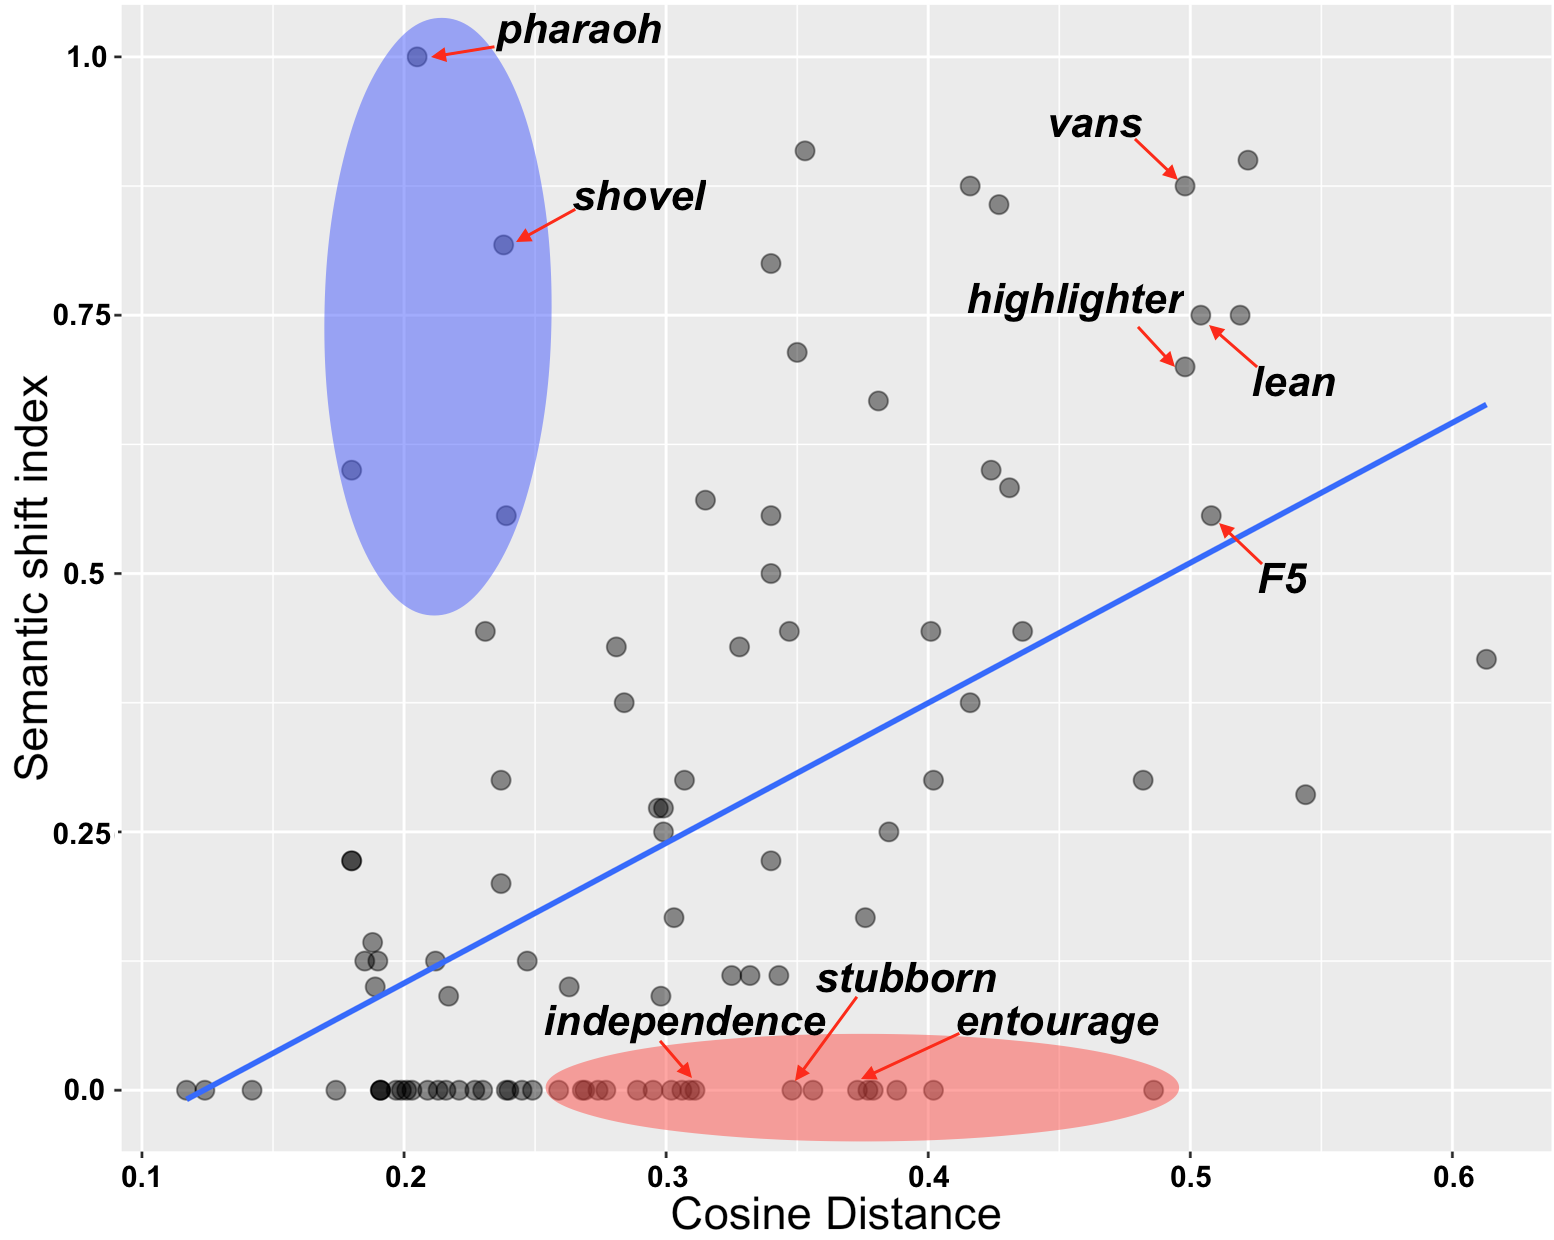
\includegraphics[width=\columnwidth]{images/cosine_distance_shift_index_annotated_3.png}
%\caption{Semantic shift index vs.~cosine distance for all words in the evaluation dataset (Pearson's $r$ = 0.49, $p< 0.001$). 
%Red ellipsis indicates false positives, blue ellipsis false
%negatives.
%\label{fig:shift-cosine}}
%\end{figure}

% RAQ's VERSION

\begin{figure}[t]\centering
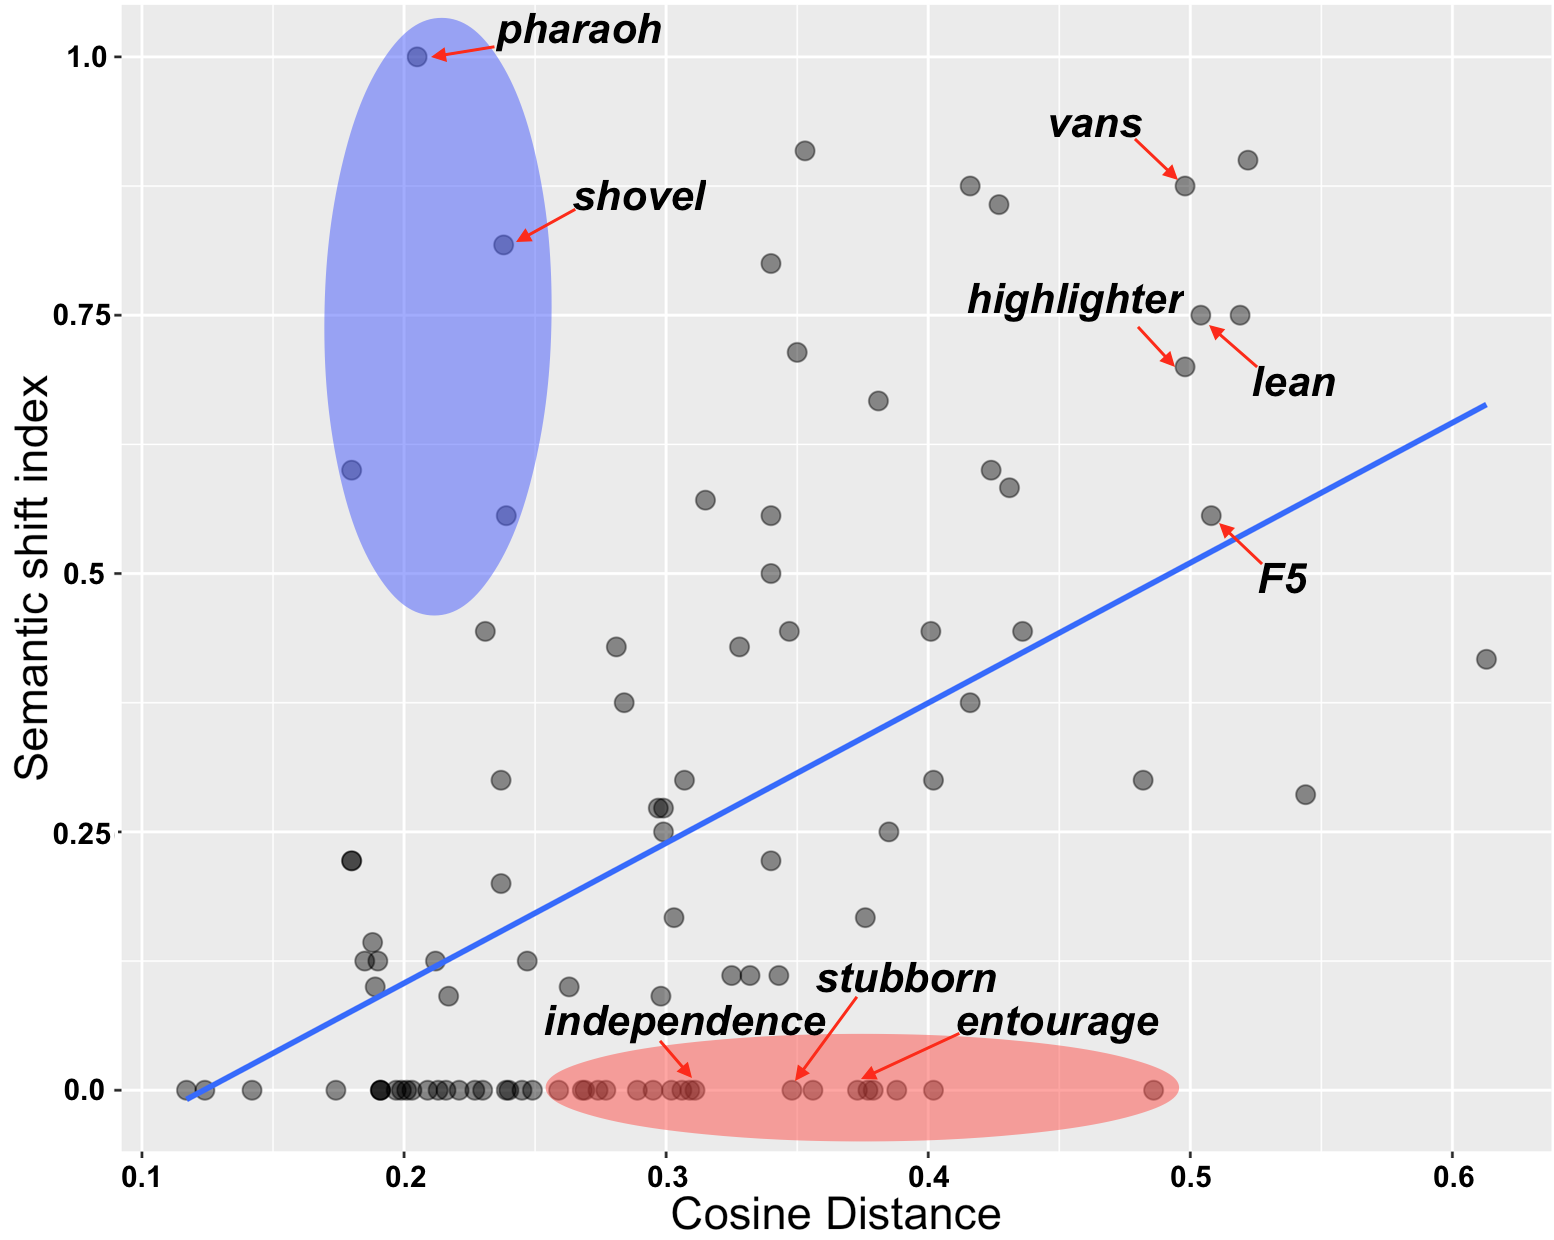
\includegraphics[width=\columnwidth]{images/cosine_distance_shift_index_annotated_3.png}
\caption{Semantic shift index vs.~cosine distance in the evaluation dataset (Pearson's $r$ = 0.49, $p< 0.001$). 
Red ellipsis:~false positives; blue ellipsis:~false negatives.
\label{fig:shift-cosine}}
\vspace*{-5pt}
\end{figure}

While the general tendency is in line with our expectations, we
also find systematic deviations. 

\paragraph{False negatives.}
A small, but consistent group is that of %\textit{false negatives}: 
words that undergo semantic shift but are not captured by the model
(blue ellipsis Figure~\ref{fig:shift-cosine}; shift index\textgreater 0.5, cosine distance\textless 0.25).
These are all metaphorical shifts; in particular, cases of extended
metaphor \cite{werth1994extended}, where the metaphor is 
developed throughout the whole text produced by an author. For instance, besides the {\em `shovel'} example mentioned in Section~\ref{sec:types}, we find the word {\em `pharaoh'} as the nickname of an Egyptian player who
joined Liverpool in 2017, used in
sentences like \textit{`approved by our new Pharaoh Tutankhamun'}, or \textit{'our dear Egyptian Pharaoh, let's hope he becomes a God'}.
Despite the metaphoric usage, the local context of these words is similar to the literal one, and so the model does not spot the meaning shift. We expect this to happen in long-term shift models, too, but we are not aware of results confirming this.

\paragraph{False positives.}
A larger group of problematic cases is that of %\textit{false positives}, that is, 
words that do \textit{not} undergo semantic shift despite showing
relatively large differences in context between $t_1$ and $t_2$ (red ellipsis in
Figure~\ref{fig:shift-cosine}; shift index=0, cosine distance\textgreater	
0.25). Manual inspection reveals that most of these ``errors'' 
are due to a referential effect: words are used
almost exclusively to refer to a specific person or event, and
so the context of use is different from the contexts in $t_1$.
%\todo{M:this is dangerous, cause we do not prove this} 
For instance, {\em `stubborn'} is
almost always used to talk about a coach who was not
there in 2013 but only in 2017; 
{\em `entourage'}, for the entourage of a particular star of the team; {\em `independence'} for the
political events in Catalonia (Spain). 
In all these cases, the meaning of the word stays the same, %\todo{R: should we say the *ontological* meaning stays the same?} 
despite the change in context. In line with the Distributional
Hypothesis, the model spots the context change, but it is not
sensitive to its nature. We expect long-term shift to not be as
susceptible to referential effects 
like these because
embeddings are aggregated over a larger and more varied number of
occurrences.

We expect that in referential cases the contexts of use will not
simply be different, but \textit{narrower} than for words with actual
semantic shift, because they are specific to one person or
event. Hence, using a measure of \textit{contextual variability}
should help spot false positives.  To test this hypothesis, we define
contextual variability as follows: for a target word, we create a
vector for each of its contexts (consisting of 5 words to the left and
to the right of the target) in $t_2$ by averaging the embeddings of
the words occurring in it, and define variability as the average
pairwise cosine distance between context vectors.  We find that
contextual variability is indeed significantly correlated with
semantic shift in our dataset (Pearson's $r\!=\!0.55$, $p\!<\!0.001$),
while it is independent from cosine distance (Pearson's $r$= 0.18,
$p> 0.05$). These two aspects are thus complementary. While both shift
words and referential cases change context of use in $t_2$, context
variability captures the fact that only in referential cases words
occur in a restricted set of contexts. The scatterplot in
Figure~\ref{fig:shift-variability} shows this effect visually.  This
result can inform future computational models of short-term meaning
shift.
% gbt: if anything, this should go in the conclusion, but I'd leave it out
% In future work, we plan to investigate more in depth the interplay between variability, cosine and semantic shift, both in short- and long-term meaning change.

\begin{figure}[h!]\centering
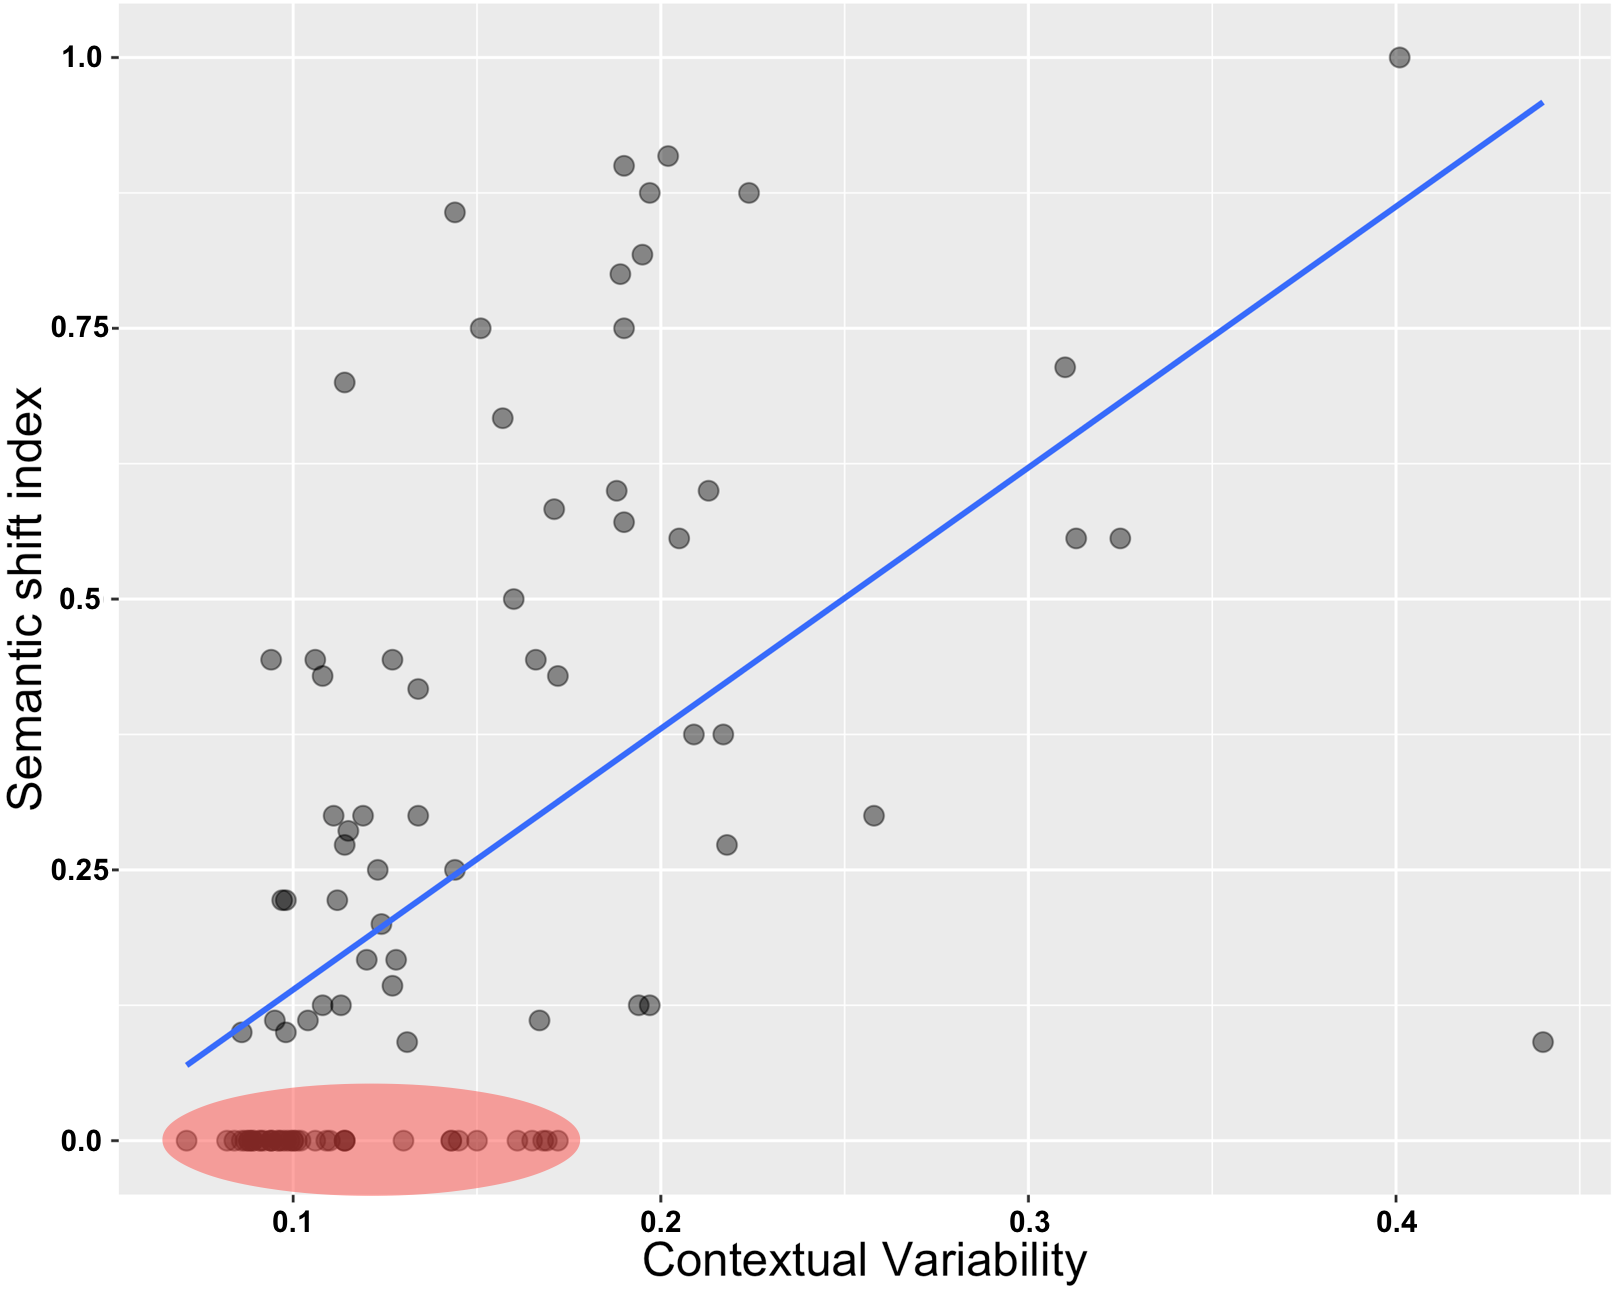
\includegraphics[height=4.3cm]{images/contextual_variability_shift_index_annotated_2.png}
\vspace*{-2pt}
\caption{Semantic shift index vs.~context variability. Red ellipses: referential cases which are assigned high cosine distance values by the model (false positives).\label{fig:shift-variability}}
\vspace*{-5pt}
\end{figure}


%\begin{figure}[t]\centering
%%\includegraphics[width=\columnwidth]{graph_and_csv/plots/shift-cosine-correlation-plot.png}
%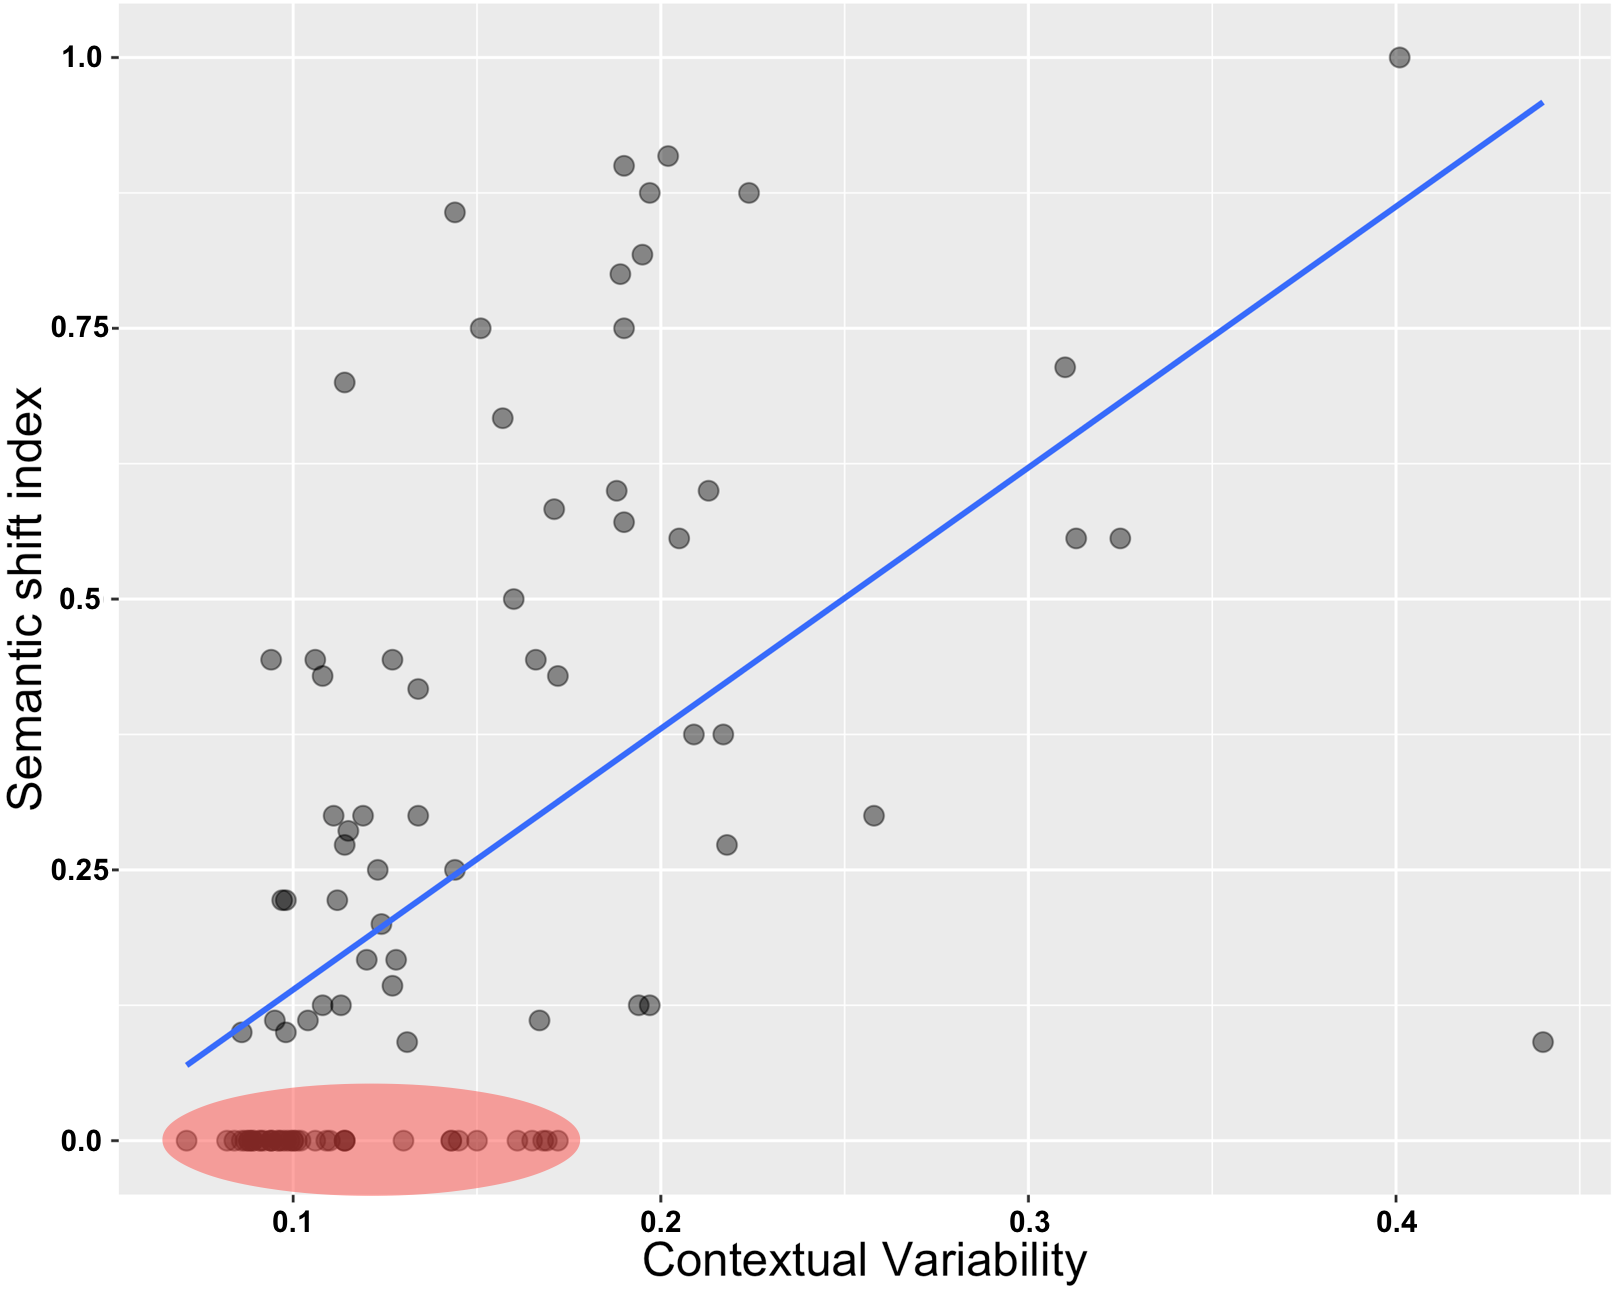
\includegraphics[width=\columnwidth]{images/contextual_variability_shift_index_annotated_2.png}
%\caption{Semantic shift index vs.~context variability for all words in the evaluation dataset (Pearson's $r$ = 0.55, $p< 0.001$). Red ellipses indicates the referential cases which are assigned high cosine distance values by the model (false positives).
%\label{fig:shift-variability}}
%\end{figure}


%




%% PREVIOUS VERSION


%Although the general tendency is in line with our expectations, we
%also find systematic deviations. First, \textit{false positives}, that
%is, words that do not undergo semantic shift despite showing
%relatively large differences in context between $t_1$ and $t_2$ (red ellipsis in
%Figure~\ref{fig:shift-cosine}; shift index=0, cosine distance\textgreater	
%0.25). 
%%\todo{G Redraw red ellipsis to cover fewer datapoints -- maybe  higher than 0.25? Else too close to the 0 x-axis.}
%Manual inspection reveals that most of these ``errors'' 
%%\todo{Add  number (X out of Y)?} 
%are due to a referential effect: words are used
%% \paragraph{False Positives.}
%% The analysis of words in this group reveals that, indeed, they occur
%% in a different context in $t$ 2 compared to  $t$ 1: however, this not
%% due to a meaning shift, but rather to the fact that they are used 
%almost exclusively to refer to a specific person or event, and
%so the context of use is narrowed down with respect to $t_1$.
%%\todo{M:this is dangerous, cause we do not prove this} 
%For instance, `stubborn' is
%almost always used to talk about a coach who was not
%there in 2013 but only in 2017; 
%%`village', for the village in Africa where one of the new players comes from; 
%`entourage', for the entourage of one of the stars of the team; `independence' for the
%political events of Catalonia (Spain). 
%%\todo{do we want to include the example  of `parked'?}. 
%% the target word is temporary
%% narrowing down its context of use to refer to a specific referent, but
%% without a semantic shift.
%In all these cases, the meaning of the word stays the same, despite
%the change in context. In line with the Distributional Hypothesis, the model spots the change, but it is not sensitive to its nature.
%Long-term shift is not as sensitive to changes of referential nature
%like these because
%embeddings are aggregated over a larger and more varied number of
%occurrences.
%%However, with small time-scales and in-community semantic shift, this problem clearly emerges.
%
%%\raq{To structure this, now I would add two subheadings (with paragraph command) for false positive and false negatives and put the explanations/examples you have below for each of them.}
%
%
%A smaller, but consistent group is that of \textit{false negatives}, 
%words that undergo semantic shift but are not captured by the model
%(blue ellipsis; shift index\textgreater 0.5, cosine distance\textless 0.25).
%%: `dilly', `shovel', `shovels', `pharaoh'.\todo{M: dont't think list is necessary}
%%\gbt{List the  words here, since they are only 4.}
%%\paragraph{False Negatives.}
%%On the top left of the plot cluster cases that can be considered as
%%\textit{false negatives}, i.e. words that are considered cases of
%%semantic shift by the redditors (high semantic shift index values),
%%but not by the model (low cosine distance). 
%\gbt{To do: move this to the ling analysis section, and here only link?} \marco{don't know, I see it more here maybe. Raq?}
%These are cases of \textit{extended}
%metaphor \cite{werth1994extended}, that is, cases in which the metaphor is 
%%not limited to a single word, but it is 
%developed throughout the whole text produced by an author. Also in this case, the model ``is right'', in the sense that indeed
%the local context of the target words does not change in $t_2$.
% % As a result, the context taken into consideration by the model is
% % indeed the one in which the word normally occurs, and for this
% % reason the model is not able to spot the meaning shift. 
%For instance, `pharaoh' is the nickname of an Egyptian player who
%joined Liverpool in 2017 and is used in
%sentences like \textit{`approved by our new \textbf{Pharaoh}
%  Tutankhamun'}, \textit{'our dear Egyptian \textbf{Pharaoh},
%  let's hope he becomes a God'}, and so on. Similarly, `shovel',  occurs in sentences
%like \textit{`welcome aboard, here is your \textbf{shovel}'},
%\textit{`you boys know how to \textbf{shovel} coal'}: the team is seen as a train that is running through the season, and every supporter is asked to give its contribution, depicted as the act of shoving coal into the train boiler. Despite the metaphoric usage, the local context of these words is similar to the literal one, and so the model does not spot the meaning shift. We expect this to happen in long-term shift models, too, but we are not aware of results confirming this.
%



%\section{Contextual variability}
%
%From the analysis it emerges that the main issue for distributional models when dealing
%with short-term shift is contextual change due to referential aspects (false positives).
%We expect that in referential cases the context of use will be
%\textit{narrower} than for words with actual semantic shift, because
%they are specific to one person or event. Hence, using a measure of
%\textit{contextual variability} should help spot false
%positives.
%Here we test this hypothesis. 
%We define contextual variability as follows: for a target word, we create a vector for each of its contexts in $t_2$ by averaging the embeddings of the words  occurring in it, and define variability as the average pairwise cosine distance between context vectors.\footnote{We consider the context as the five words occurring on the left and on the right of the target word.}We then test whether contextual variability has explanatory power over cosine distance by fitting a linear regression model with these two variables as predictors and semantic shift index as dependent variable.\footnote{Contextual variability and cosine distance are not correlated in our data (Pearson's $r$= 0.18,$p> 0.05$). }
%The results indicate that these two aspects are indeed complementary
%(contextual variability: $\beta$= 0.47, $p< 0.001$, cosine distance:
%$\beta$= 0.40, $p< 0.001$, adjusted $R^2$=0.44). While both shift
%words and referential cases change context of use in $t_2$, context
%variability captures the fact that only in referential cases words
%occur in a restricted set of contexts. The scatterplot
%\ref{fig:shift-variability} shows this effect visually. \new{This result can inform future models of short-term meaning
%  shift.} \textcolor{red}{In future work, we plan to investigate more in depth the interplay between variability, cosine and semantic shift, both in short- and long-term meaning shift.}\marco{I'd move this to Conclusions}



%%% Local Variables:
%%% mode: latex
%%% TeX-master: "main"
%%% End:


%============================
\section{Conclusion}
\label{sect:conc}

The goal of this preliminary study was to bring to the attention of the NLP community short-term meaning shift, an under-researched problem in the field. 
% gbt: in a short paper we don't need a recap
% Our contribution is twofold: (i) we create and make available a dataset for short-term meaning shift manually annotated by experts; (ii) we test the performance of a standard model for diachronic meaning shift on such a dataset, providing a detailed error analysis that provides insights into the phenomenon.
We hope that it will spark further research into a phenomenon which, besides being of theoretical interest, has potential practical implications for NLP downstream tasks concerned with user-generated text, as modeling how words meaning rapidly change in communities would allow to better understand what their members say.




\bibliography{naaclhlt2019}
\bibliographystyle{acl_natbib}

%\appendix

\end{document}

%%% Local Variables:
%%% mode: latex
%%% TeX-master: t
%%% End:

